\section{Approach}
\label{sec:approach}
In this section, we first introduce the general framework of ChatMatch, which is modeled as
a sports tournament, then discuss some possible scoring metrics (or dimensions) 
that can be used by the virtual judges in these matches. 

%Our whole evaluation framework consists of competition and scoring at three different levels. 
%The game level is at the bottom 
%and is played between two players. 
%Then comes the match level.
%To ensure the fairness of the game, 
%two games will be played between every two robots, 
%with each side starting a conversation.
%The result of two games determines the outcome of a match. 
%The tournament level is at the top
% and is composed of matches among different pairs of players. 

\subsection{Competition Protocol}
\label{sec:competition}
The competition takes place, from top to bottom, at tournament, match and
game levels.

\subsubsection{Tournament Rules}
%\KZ{Give an overview of the how the tournament is run.}
We adopt a double round-robin 
sports tournament, where all bots participating in the competition 
converse directly with each other twice.
This is better than a knock-out system because it assesses a bot's ability to
deal with both strong and weak bots.
%For example, whether with weaker bots will induce them to make more mistakes or  how stronger bots will motivate their performance.
If there are $n$ chatbots to be evaluated, 
there will be $n \choose 2$ matches in total.

\subsubsection{Match Rules}
%\KZ{Talk about how the matches are administered. Just the procedure only.}
Each match happens between two bots and consists of two games,
each started by a different bot. Thus for $n$ bots, there are
$n \times (n-1)$ games in total. 

\subsubsection{Game Rules}
%\KZ{The procedure of the game. How each game is started and stopped.}
Each game is started by a player whose first utterance is provided by 
the system. The choice of the first utterance can be different 
depending on the domain of the bots and the ability we want to 
rank about the bots. For example, if we want to test 
the ability on movies, we can set a movie-related 
first utterance. To end the conversation, 
%there might be different ways to 
%end the conversation. 
we set a fixed number of exchanges~\footnote{An exchange of conversation is two turns, one from each speaker.} 
%or a terminating condition such as whether a bot makes a fatal error
%or whether a certain score is reached. \KZ{What is a fatal error? If we never
%elaborate this idea later in the paper, better not mention it at all.
%This can make our approach difficult to follow.}

%We acknowledge that there exists other complex and advanced 
%competition protocols, such as knock-off or Swiss system tournament, 
%but the double round-robin system used here is simple and can 
%deal with any number of bots. \KZ{Check the above if it's correct.} 

\begin{table*}[th]
\centering
%\scriptsize
\small
\begin{tabular}{c|l|l}
%\hline
\toprule
\textbf{Dimension} & \textbf{Definition} &\textbf{Approach} \\ \midrule
Fluency  & Responses are fluent and natural.& Sentence perplexity. \\
Knowledge & Responses indicate the bot has the & Inspired by \citet{finch-choi-2020-towards}, we count the number \\
&knowledge. &of entities per hundred exchanges. \\
%\KZ{The number of times the bot expresses its ignorance to a question.} \\
%& & \KZ{(e.g., answering ``I don't know'' to a question.)}\\
Proactivity & Responses actively proceed the conversation.&The number of times the bot raises a question. \\
Specificity & Responses are not generic.&The average of Distinct-1 and Distinct-2 \citep{li-etal-2016-diversity}.\\
Diversity &Responses are diverse and non-repetitive. &Repetition detection following the function in \algoref{algo:rep}. \\
Consistency &Responses do not contradict chat history. &Detect inconsistency following the function in \algoref{algo:inconsist}\\
Relevance & Responses are relevant to current context.& Detect 
relevant concepts in chat history as in \algoref{algo:bonus}. \\
\bottomrule
\end{tabular}
\caption
\label{tab:methods}
\end{table*}


\subsection{Scoring}
\label{sec:scoring}
\subsubsection{Game-level Scoring}
%\KZ{Define a few functions: one to catch repeating, one to chat contradiction and one to catch long term memory.}

%Here we define the rules for recording points in one game between two bots. 
Inspired by \citet{finch-choi-2020-towards}, 
we score each dialogue turn based on seven aspects: 
\textit{consistency}, \textit{fluency}, \textit{knowledge}, \textit{specificity}, 
\textit{diversity}, \textit{relevance} and \textit{proactivity}.
\tabref{tab:methods} documents the definition of these dimensions
and 
gives a brief view of tools that
we used for automatic evaluation. 


%which can all be scored automatically. 
%As these seven metrics present a high level of 
%overlap among all distinct evaluation metrics used 
%during different process of human evaluation,
%we believe the combination of these seven distinct dimensions will be reliable. 
%Finally, we sum up the scores for each bot for all the turns.
%\tabref{tab:methods} documents the definition of these dimensions, which can all be scored
%automatically.

%After finishing the calculation of the bonus and penalty scores for each turn, we obtain the scores of the two bots in a game with weighted sum according to \eqnref{eq:sum-up}

%\begin{equation}
%S(bot) = \sum_t - c\times C(t)  - r \times R(t) + b \times B(t)
%\label{eq:sum-up}
%\end{equation}
%$S$ denotes the total score gained by a bot for a game.
 
Fluency, Knowledge, Proactivity and Specificity are scored for each turn separately
and aggregated at the end of the conversation. 
%\tabref{tab:methods} gives a brief view of tools that 
%we used for automatic evaluation.
We choose the most widespread reference-free approach, 
perplexity, to evaluate the fluency
of each generated turn.
Following \citet{bao-etal-2021-plato}, 
we use the average of Distinct-1 and Distinct-2 \citep{li-etal-2016-diversity},
which computes the lexical variety, to approximate the specificity of a response.
As for evaluating knowledge and proactivity, we
%count the number of expressions about uncertainty (e.g., answering ``I don’t know") and the number of questions.
%\textcolor{green}{zitong:
count the number of entities and the number of questions of each bot.
%}
%\KZ{Need to clearly define ``ignorance''. 
%Did you mean that the bot say ``no'', ``i don't know'' or 
%stuff like that?}
In need of considering the context while evaluating diversity, consistency and relevance,
we propose more involved rules in \algoref{algo:rep}, 
\algoref{algo:inconsist} and \algoref{algo:bonus}.
\tabref{tab:functions} shows the symbols we use in the algorithms.

\begin{table}[th]
\centering
%\scriptsize
\small
\begin{tabular}{c|l}
%\hline
\toprule
\textbf{Notation} & \textbf{Description} \\ \midrule
$t$ & Current turn \\
$H(t)$  &  a list of history turns prior to $t$ \\
$Sim(x,y)$ & similarity between two turns $x$ and $y$ \\
$\sigma_r$ & Threshold for detecting repetition \\
$\sigma_c$ & Threshold for detecting consistency \\
$r$ & Weight for repetition \\
$c$ & Weight for inconsistency \\
$b$ & Weight for bonus \\
$d$ & Min distance between consecutive mentions \\
IDF list & List of lemma in chatlog sorted by IDF\\
$p$ & Percentage of important lemmas in IDF list\\
$R(t)$ &  Repetition penalty for turn $t$ \\
$C(t)$ &  Inconsistency penalty for turn $t$ \\ 
$B(t)$ &  Memory bonus for turn $t$ \\
$Rep(t)$ & A list of repeated turns for turn $t$ \\  
\bottomrule
\end{tabular}
\caption{
Functions and variables in algorithms.}
\label{tab:functions}
\end{table}

\begin{algorithm}[th]
\small
\caption{Scoring for Diversity}
\label{algo:rep}
\hspace*{0.02in} {\bf Input:}
 $t$, $H$, $Sim$, $\sigma_{r}$
; \hspace*{0.02in} {\bf Output: } 
 $R$;
\begin{algorithmic}[1]
\State //Starting to detect repetition
\State $R(t) \leftarrow 0$
\For {$u$ in $H(t)$}
	\If {$Sim(t,u) \geq \sigma_{r}$}
		\State Add $u$ to $Rep(t)$
	\EndIf
\EndFor
    \If{$len(Rep(t))\geq 0$}
        \If{$t$ is a question and we can find a similar question in $Rep(t)$}
        \State $ R(t) \leftarrow  R(t) + 1$ 
        \Else
        \If {the previous turn of $t$ is not a repetitive question}
        \State $R(t) \leftarrow R(t) + 1$ 
        \EndIf
        \EndIf
    \EndIf
\end{algorithmic}
\end{algorithm}


\begin{algorithm}[th]
\small
\caption{Scoring for Consistency}
\label{algo:inconsist}
\hspace*{0.02in} {\bf Input:}
$t$, $H$, $Sim$, $\sigma_{c}$
; \hspace*{0.02in} {\bf Output:  } 
 $C$;
\begin{algorithmic}[1]
\State // Inconsistency detection
\State $C(t) \leftarrow  0$
 \If {previous turn of $p$ is a repetitive question} 
   \If{ the response $res$ to the question repeated by turn $p$ contradicts turn $i$ with $Sim(t, res) \leq \sigma_{c}$ }
    \State $C(t) \leftarrow C(t) + 1$
   \EndIf
  \EndIf
\end{algorithmic}
\end{algorithm}

\begin{algorithm}[th]
\small
\caption{Scoring for Relevance}
\label{algo:bonus}
\hspace*{0.02in} {\bf Input:}
$t$, $p$, $d$
; \hspace*{0.02in} {\bf Output:  } 
$B$;
\begin{algorithmic}[1]
\State // Assessing the ability of catching relevant concepts\\
$B(t) \leftarrow 0$
\For {all tokens $tk$ in current turn $t$}
 \If {$t$ - previous occurrence turn of $tk > d$ and $tk$ in the top $p\%$ of the IDF list of all tokens in the dialogue} 
   \State $B(t) \leftarrow 1$
  \EndIf
 \EndFor
\end{algorithmic}
\end{algorithm}

%described in detail in  
%\tabref{tab:functions} and \algoref{algo:rep} through \algoref{algo:bonus}.
We use an example in \figref{fig:example}
to explain how to work with them.
We evaluate diversity by punishing
repetition in one dialogue.
 At each turn $t$, we first check if there exists any repetitive question.  
Here in \figref{fig:example},
we can easily find turn 3 and turn 7 repeated turn 1 and turn 5 
respectively. They will then be penalized one point for repetition. 
Repetition is not penalized if the previous turn is already 
marked as a repetitive question. For example, in \figref{fig:example}, 
although turn 4 is considered a repetition of turn 2,  
we are not going to penalize it as turn 3 is a repetitive question. 

\begin{figure}[th]
        \centering
        \includegraphics[width=\columnwidth]{example_log.eps}
        \caption{A chat snippet between two bots.}
        \label{fig:example}
\end{figure}

Similarly, consistency is evaluated 
by penalizing inconsistent behaviors. 
The detection of inconsistency is always triggered after the detection of repeated questions. 
If the answers to the same questions are different, we will penalize the current turn, 
such as turn 8 in \figref{fig:example}. %\KZ{One problem is that inconsistency
%will not be assessed if there's no repeated questions at all. That sounds like
%a flaw of the design. If we can insert some repeated questions (or questions
%with the same meaning) automatically into the chat, then we can test this more
%effectively.} We decide a repetition or an inconsistency by calculating the similarity of the two turns. 
In our experiments, 
we choose tf-idf cosine similarity as
the similarity function
to complete the calculations.
% which we will 
%discuss in \secref{sec:experiment}. 
The actual diversity and consistency scores
are the negation of the amount of repetition and inconsistency.

Relevance is assessed as a bonus to reward
a bot if it is able to memorize the important relevant concepts that have shown up 
before in the conversation. We sort the concepts that have shown up in 
chat history by their IDF scores. For example, in turn 9, $A$ 
mentions the concept word ``student'' presented by $B$ in turn 2. With this
turn, $A$ will win a bonus point.

At the end of each game, each bot gets seven raw scores, 
one for each dimension.  
A bot receives one point on a dimension if it gets a higher raw score 
compared with the other bot in the game and zero point otherwise. 
The final score
of each game 
for each bot is the sum of the points on these seven dimensions,
which will not surpass 7.
%The sum of the final scores of these two bots will be 7. 
%\KZ{Are these scores positive or negative? Comparable between bots?}
\subsubsection{Tournament-level Scoring}
%\subsubsection{Match-level Scoring}
%\textcolor{red}{we don't need this subsection as we use trueskill now.
%BTW, Reviewer 1 said that:Section 2.2.3: As someone not familiar with tournament ranking schemes, I would like to see this section expanded a bit to explain in more detail how TrueSkill works. }
%\KZ{Use an equation to compute the final scores?}
One naive method for adding up the scores which come from each game is to mimic the
rules of sports tournaments: 
one match which consists of two games, each started with a different bot, 
decides winning or losing between two bots.
%For match-level scoring, 
%we then the scoring rules of soccer tournaments: 
Then for each match, we score $W$ points for the winner,  
$T$ points for a tie and 
$L$ points for the loser.
The value of $W$, $T$ and $L$ will be discussed in \secref{sec:ablation}. 
For Tounrnament level, 
we count the points by summing up the scores gained in every match.
%\KZ{At the match level, we need to consider different starting context for the bots? I think we should present a few options for the reader and say that we are limited to these.}
%\subsubsection{Tournament-level Scoring}
%\KZ{Use an equation to compute the final scores?}
%We count the points by summing up the scores gained in every match. 
%In this work, several bots can have identical final scores which means they
%are tied. For future study, it's possible to mimic more complex
%rules present in sporting matches, e.g., determine their ranking based on 
%their win-loss relationship in the match between them.  
%If they are still tied, we can propose an ``overtime'' match for these 
%two bots, one human judge may observe their performance and then 
%make the final decision.

Another choice is to use TrueSkill \citep{herbrich2007trueskill} algorithm to rank them. 
TrueSkill system is a ranking system which is based on Bayesian inference.This scoring system
takes into account the uncertainty of each chatbot by considering 
their winning percentage and possible fluctuations.
In this algorithm, the ability of each bot is regarded as a normal distribution. Each game result leads to an update of the bots' ability. %Different game order may lead to different results and the rankings will converge after a certain number of matches. 
In order to guarantee a stable ranking, we randomly shuffle the order of the game three times and get the final ranking on average.
